\chapter{RESULTS AND DISCUSSION}

\section{Introduction}

The findings of this research and comprehensive discussion on TerraNode system is provided in this chapter and compared against the requirements set in Chapter Three. The chapter is organised around the four specific research aims of the study. The research results are presented under each objective: Objective One is detailing the backend architecture (mathematical modelling, algorithmic workflow, and user interface dashboards), Objective Two is detailing the predictive analytics module (mathematical modelling, algorithmic workflow, and interactive user interface), Objective Three is detailing the blockchain security and cryptographic pipeline (execution benchmarks, comparison with existing literature, and architecture diagrams), and Objective Four is detailing a comprehensive empirical evaluation of functional testing, security resilience, blockchain throughput, and API latency. The results of the research are discussed as per the core research questions and literature reviewed in Section \ref{sec:discussion}. A summary of the chapter is included in Section~\ref{sec:ch4_conclusion}. In Appendix~\ref{app:code_listings}, the code for important algorithms is included.

\section{Research Results}
\label{sec:research_results}

\subsection{Research Objective One (1): Web-Based Agricultural Data Management Platform}

The first research goal is to develop a web based agricultural data management system to collect, store and present environment and production information. The goal was achieved by creating a module based Django REST backend, an asynchronous RESTful API and a modern React-based frontend which offers customisable dashboards for all stakeholders in the agricultural value chain.

\subsubsection*{Backend Architecture and API Implementation}

The TerraNode backend is written in Django and the Django REST Framework (DRF) and is structured into four separate domain modules:

\textbf{Users Module:} Responsible for managing users' registration, credential authentication, role assignment and cryptographic wallet binding. Custom user model that adds an email-based authentication and a 66-character hexadecimal Sui wallet public key field to Django's \texttt{AbstractUser} class. This module contains five endpoints for credential login, Sui wallet login, token refresh, registration, and logout. Limits login attempts to 5 attempts per minute per IP address.

Telemetry Module: Collects, checks and records environmental sensor readings. The incoming payload is checked for the following conditions: temperature ranges from $-50^\circ$C to $100^\circ$C, relative soil moisture ranges from $0.0\%$ to $100.0\%$ and soil pH ranges from $0.0$ to $14.0$. A cryptographic digest (SHA-256) is generated for each valid reading before it is inserted into the database. A unique database constraint exists on hash to avoid duplicates.

The Ledger Module is responsible for managing the lifecycle of agricultural produce batches between the off-chain database and on-chain Sui distributed ledger. The two-phase commit protocol is used: the farmer stages a batch in \texttt{PENDING} status using the Prepare endpoint and then completes the on-chain minting transaction on their connected wallet, then submits the resulting Sui Object Identifier (UID) and transaction digest using the Confirm endpoint to mark the batch as \texttt{MINTED}.

\textbf{Analytics Module:} Performs crop yield forecasting algorithms on historical telemetry data. The prediction service fetches the telemetry points, calculates weighted moving averages, calculates a variance adjusted confidence score and provides a practical agronomic recommendation. For optimization, computed forecasts are stored in Redis with a 10 minute (600 seconds) expiry time (TTL).

Table~\ref{tab:api_endpoints} outlines the primary version-prefixed RESTful API endpoints.

\begin{table}[H]
\centering
\small
\singlespacing
\renewcommand{\arraystretch}{1.15}
\caption{TerraNode RESTful API Endpoint Structure}
\label{tab:api_endpoints}
\begin{tabularx}{\textwidth}{|l|l|>{\raggedright\arraybackslash}X|}
\hline
\textbf{Endpoint Prefix} & \textbf{Application} & \textbf{Key Functional Endpoints} \\
\hline
\texttt{/api/v1/auth/} & Users & \texttt{login/}, \texttt{wallet-login/}, \texttt{register/}, \texttt{refresh/}, \texttt{logout/} \\
\hline
\texttt{/api/v1/telemetry/} & Telemetry & \texttt{submit/}, \texttt{history/}, \texttt{latest/} \\
\hline
\texttt{/api/v1/ledger/} & Ledger & \texttt{prepare/}, \texttt{confirm/}, \texttt{transfer/}, \texttt{list/}, \texttt{detail/} \\
\hline
\texttt{/api/v1/analytics/} & Analytics & \texttt{predict/}, \texttt{summary/} \\
\hline
\end{tabularx}
\end{table}

\subsubsection*{Frontend Architecture and User Interface Presentation}

The application's frontend is built as a Single Page Application (SPA) using React 19, TypeScript, and Vite. The system architecture does not allow unauthorized role hopping by using clientside role guards. Global state is implemented with React Context API, with the JWT lifecycle and session persistence handled by \texttt{AuthContext} and the Sui wallet interactions by \texttt{WalletContext} provided by Mysten Labs dApp Kit.

It offers role-specific user interfaces tailored for easy interaction between different stakeholders in the agriculture sector, including the authentication of credentials and integration with Web3 Sui wallets. In this part, the major operating interfaces that implement the system's security, anchoring of blockchain, and transfer of custody are presented.

The Farmer Dashboard is the main operational monitoring tool available for agricultural production shown in \figref{fig:farmer_dashboard}. The interface shows real-time telemetry metric cards for the micro-climate data, soil temperature, soil moisture, and soil pH, as well as active batches of produce linked to the Sui blockchain, and dynamic yield forecast summaries.

\begin{figure}[H]
    \centering
    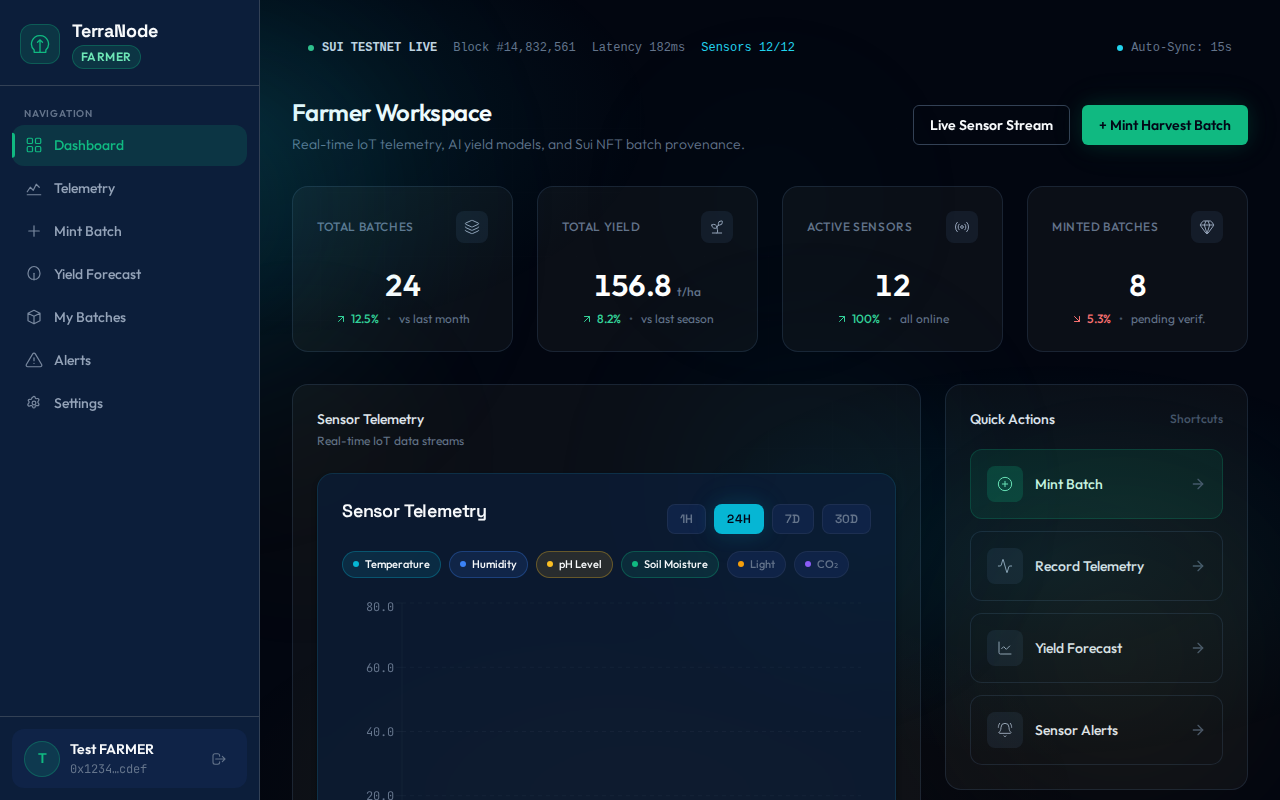
\includegraphics[width=0.88\textwidth]{figures/ui-screenshots/fig_farmer_dashboard.png}
    \caption{Farmer Operational Dashboard Displaying Real-Time Micro-Climate Telemetry and Produce Batches}
    \label{fig:farmer_dashboard}
\end{figure}

The Custody Transfer interface for logistics handlers to document physical produce transfers is provided in \figref{fig:transfer_page}. The interface records information related to the movement of the transport equipment (vehicle fleet registration, driver identity, destination terminal), then calls \texttt{agri\_ledger::transfer\_custody} on-chain to transfer the custody to the wallet address of the transport company, which guarantees the transparency of the movement's multi-hop traceability.

\begin{figure}[H]
    \centering
    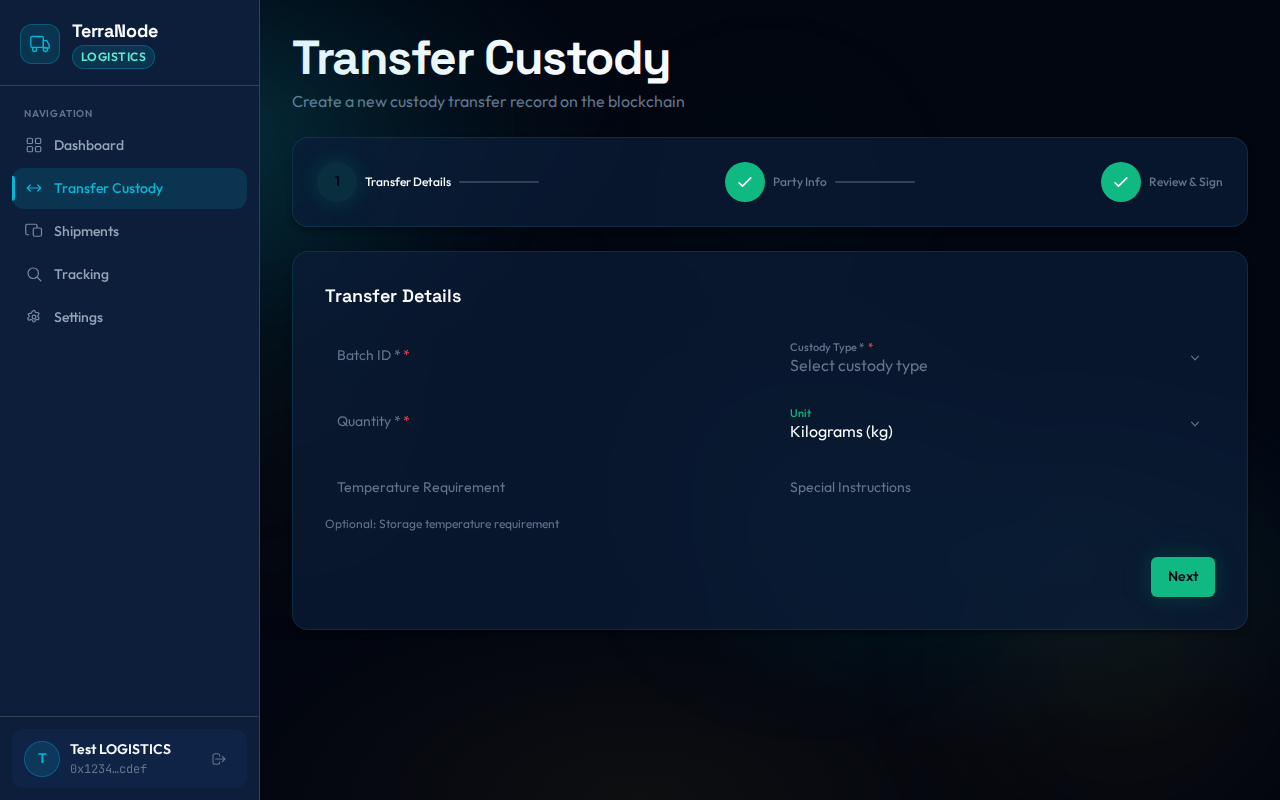
\includegraphics[width=0.88\textwidth]{figures/ui-screenshots/fig_transfer_page.png}
    \caption{Generate Custody Transfer and Blockchain Verification Interface}
    \label{fig:transfer_page}
\end{figure}

The graph in \figref{fig:audit_logs_page} shows the Administrator Audit Log, which is a rolling, tamper-evident log of all actions performed on the system, authentication attempts, and transactions performed on the blockchain. Each entry is signed with a cryptographic signature from an originating user UUID, IP address, timestamp and a SHA-256 digest for regulatory compliance and audit verification.

\begin{figure}[H]
    \centering
    
\includegraphics[width=0.80\textwidth]{figures/ui-screenshots/fig_audit_logs_page.png}
    \caption{Chronological Cryptographic Audit Log and System Activity Interface}
    \label{fig:audit_logs_page}
\end{figure}

\subsection{Research Objective Two (2): Predictive Analytics Module for Crop Yield Forecasting}

The second research goal was to design an analytics module which integrates predictive models for agricultural forecasting and decision support. This objective was met by adopting a statistical weighted moving average (WMA) prediction engine, variance indexing and dynamic confidence scoring, as well as an interactive analytics user interface.

\subsubsection*{Mathematical Modeling and Analytics Workflow}

The analytics engine takes a rolling window of time of historical telemetry data, where $n \le 90$ and $n \ge 5$. Telemetry points are pulled from the database, checked for the correct SHA-256 hash, and broken down into $T_i$ (temperature), $M_i$ (soil moisture), and $P_i$ (soil pH) feature vectors.

The arithmetic means $\bar{T}$, $\bar{M}$, and $\bar{P}$, are calculated using Equation~\ref{eq:mean_calc}:
\begin{equation}
\bar{T} = \frac{1}{n}\sum_{i=1}^{n} T_i, \quad \bar{M} = \frac{1}{n}\sum_{i=1}^{n} M_i, \quad \bar{P} = \frac{1}{n}\sum_{i=1}^{n} P_i
\label{eq:mean_calc}
\end{equation}

Crop yield $\hat{Y}$ is modelled using Equation~\ref{eq:yield_model} (in metric tons):
\begin{equation}
\hat{Y} = \max\left(0, \; \alpha + \beta_1 \bar{M} - \beta_2 |\bar{T} - T^*|\right)
\label{eq:yield_model}
\end{equation}
$T^* = 22.0^\circ$C, the optimum ambient growing temperature; $\alpha = 50.0$ is a base yield; and, $\beta_1 = 0.50$ is a positive moisture scaling coefficient, and, $\beta_2 = 1.20$ is the temperature penalty factor.

The sample variance $V$ of the environmental features is calculated to measure the degree of reliability of the prediction:
\begin{equation}
V = \frac{1}{n}\sum_{i=1}^{n} (T_i - \bar{T})^2 + \frac{1}{n}\sum_{i=1}^{n} (M_i - \bar{M})^2
\end{equation}

The confidence score $C \in [50.0\%, 95.0\%]$ is dynamically corrected following Equation~\ref{eq:conf_score}:
\begin{equation}
C = \min\left(95.0, \; \max\left(50.0, \; 95.0 - 0.05 \cdot V\right)\right) \times \min\left(1.0, \; \frac{n}{30}\right)
\label{eq:conf_score}
\end{equation}

The end-to-end architecture and the decision flow of the predictive analytics engine is shown in \figref{fig:prediction_analytics}.

\begin{figure}[H]
    \centering
    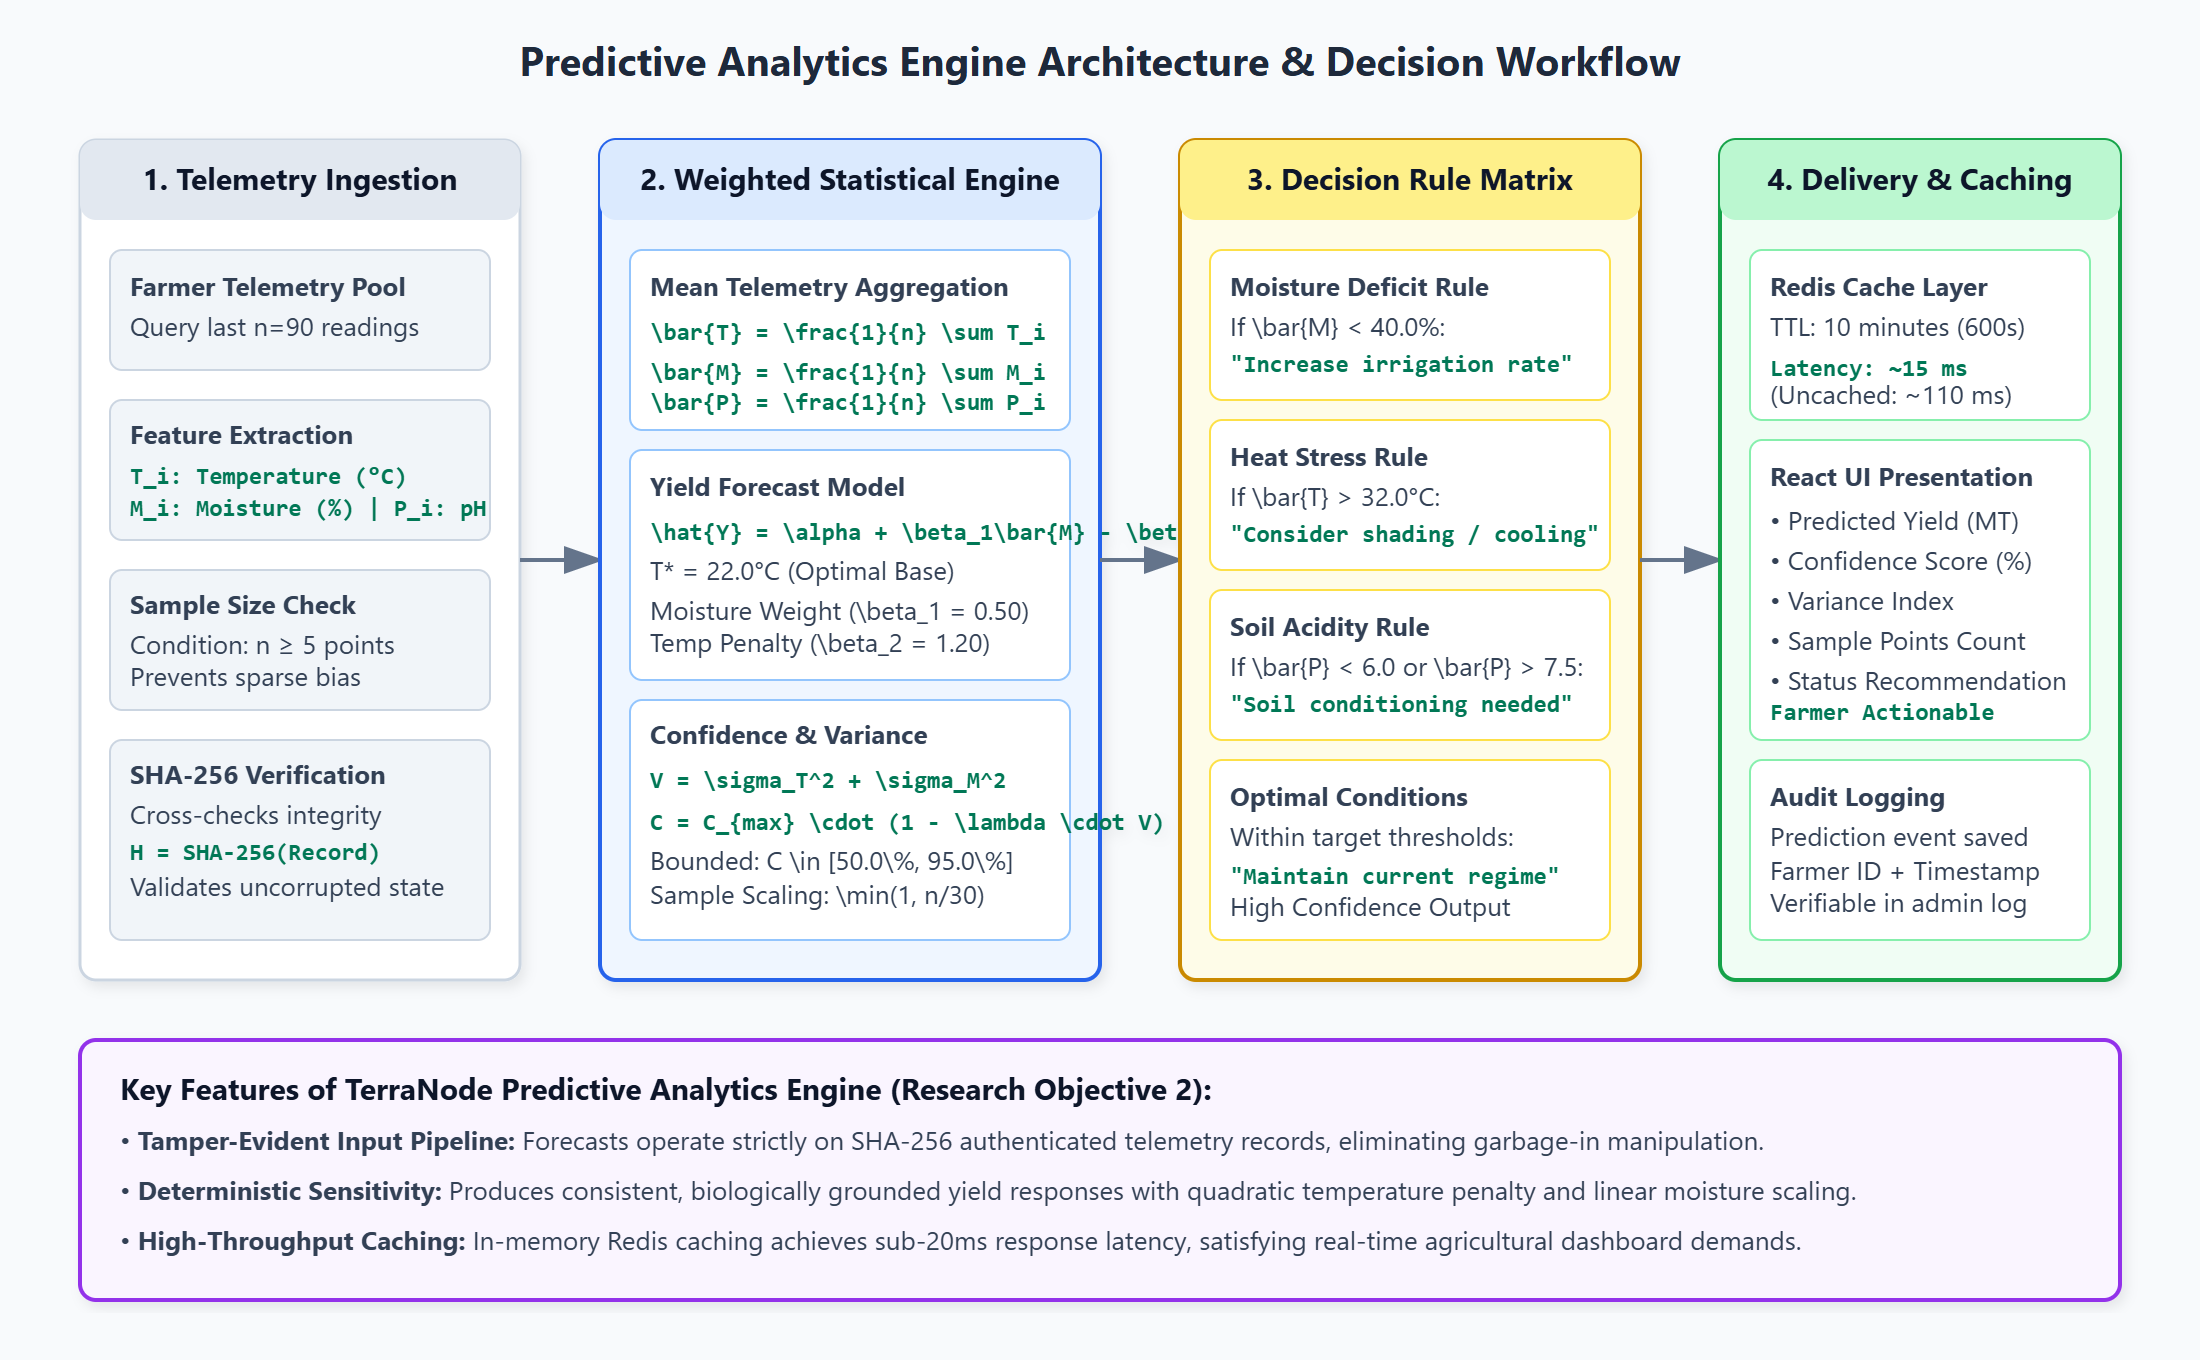
\includegraphics[width=0.95\textwidth]{figures/fig_prediction_analytics.png}
    \caption{Predictive Analytics Engine Architecture and Decision Workflow}
    \label{fig:prediction_analytics}
\end{figure}

\subsubsection*{Analytics User Interface and Decision Support Presentation}

\figref{fig:yield_prediction_page} presents the operational yield prediction and decision support interface. The interface brings to life the mathematical formulation of the model described in the Equations~\ref{eq:mean_calc}--\ref{eq:conf_score} and presents the estimated crop yield in metric tons, the computed confidence score, the micro-climate variance index, and multi-year projection curves with dynamic uncertainty bounds and actionable agronomic recommendations.

\begin{figure}[H]
    \centering
    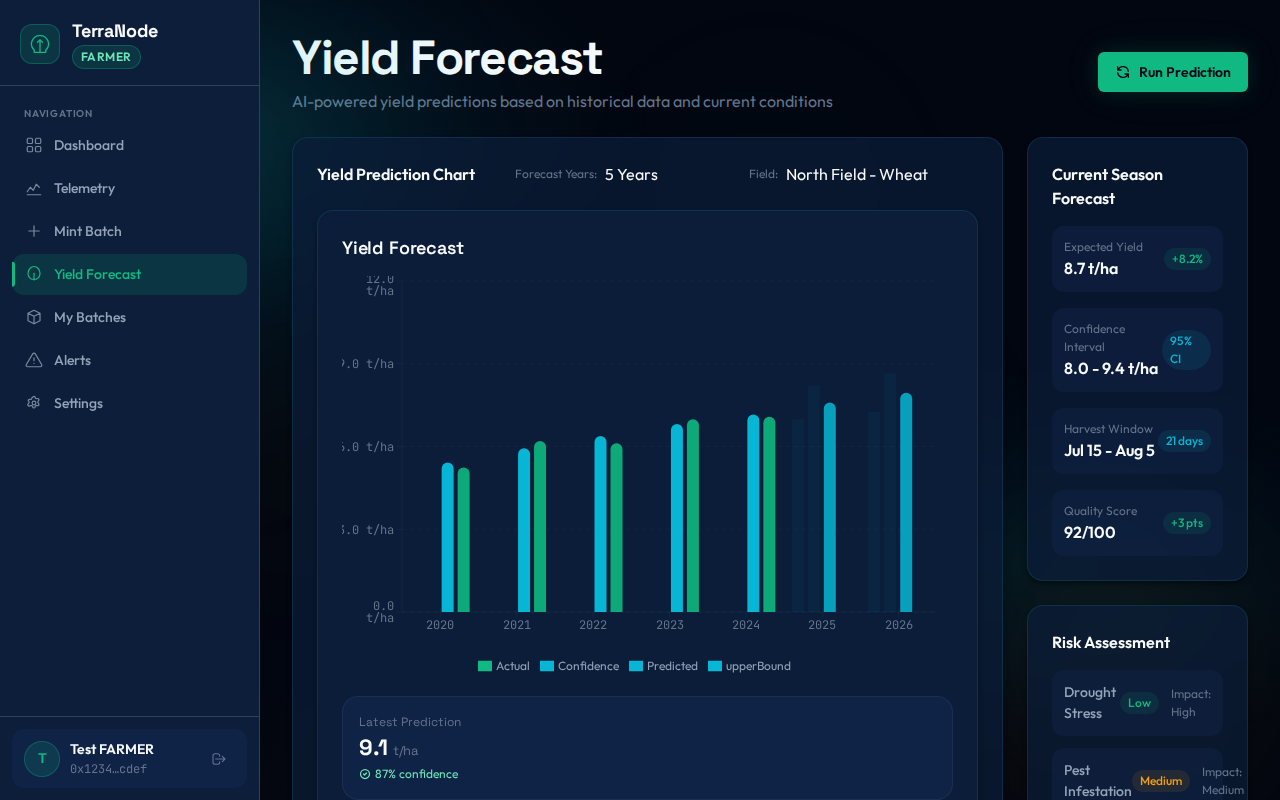
\includegraphics[width=0.88\textwidth]{figures/ui-screenshots/fig_yield_prediction_page.png}
    \caption{Yield Forecast, Soil Suitability Matrix and Decision Support Interface}
    \label{fig:yield_prediction_page}
\end{figure}

\subsection{Research Objective Three (3): Blockchain-Based Security and Cryptographic Integrity Mechanisms}

The third research goal was to develop the security mechanisms for data integrity, traceability, and unauthorized changes to agricultural records using blockchain. This goal is accomplished by a multi-layered cryptographic pipeline covering: data integrity digests using SHA-256, symmetric payload encryption using AES-256-GCM, wallet signatures using Ed25519 asymmetric signature, transaction hashing using BLAKE2b, and smart contract object anchoring on the Sui blockchain.

\subsubsection*{Cryptographic Processing Pipeline}

A cryptographic pipeline has five structured stages:
\begin{enumerate}[label=(\roman*)]
    \item The data collected in the environment is converted to a structured JSON string with farmer ID, temperature, moisture, pH, and Unix timestamps.
    \item The SHA-256 cryptographic algorithm is used to hash the serialized telemetry string to create an integrity digest of 256 bits (64 characters hexadecimal). This hash acts as the physical farm's digital ``fingerprint,'' which is unique and cannot be changed.
    \item Advanced Encryption Standard (AES) in Galois/Counter Mode (AES-256-GCM), with authenticated 128-bit MAC tag, is used for off-chain storage and secure transit of sensitive telemetry records to ensure confidentiality and cipher integrity.
    \item Ed25519 Asymmetric Digital Signing: To provide non-repudiation proof of batch origin, Sui wallet transactions are digitally signed using the Edwards-curve Digital Signature Algorithm (Ed25519: $\sigma = \text{Sign}_{sk}(\text{TxDigest})$).
    \item The \texttt{ProduceBatch} object is minted on the Sui distributed ledger, permanently associating the batch metadata with the farmer's address on the ledger and the farmer's SHA-256 hash.
\end{enumerate}

\figref{fig:crypto_pipeline} visualizes the multi-layered cryptographic and blockchain anchoring pipeline.

\begin{figure}[H]
    \centering
    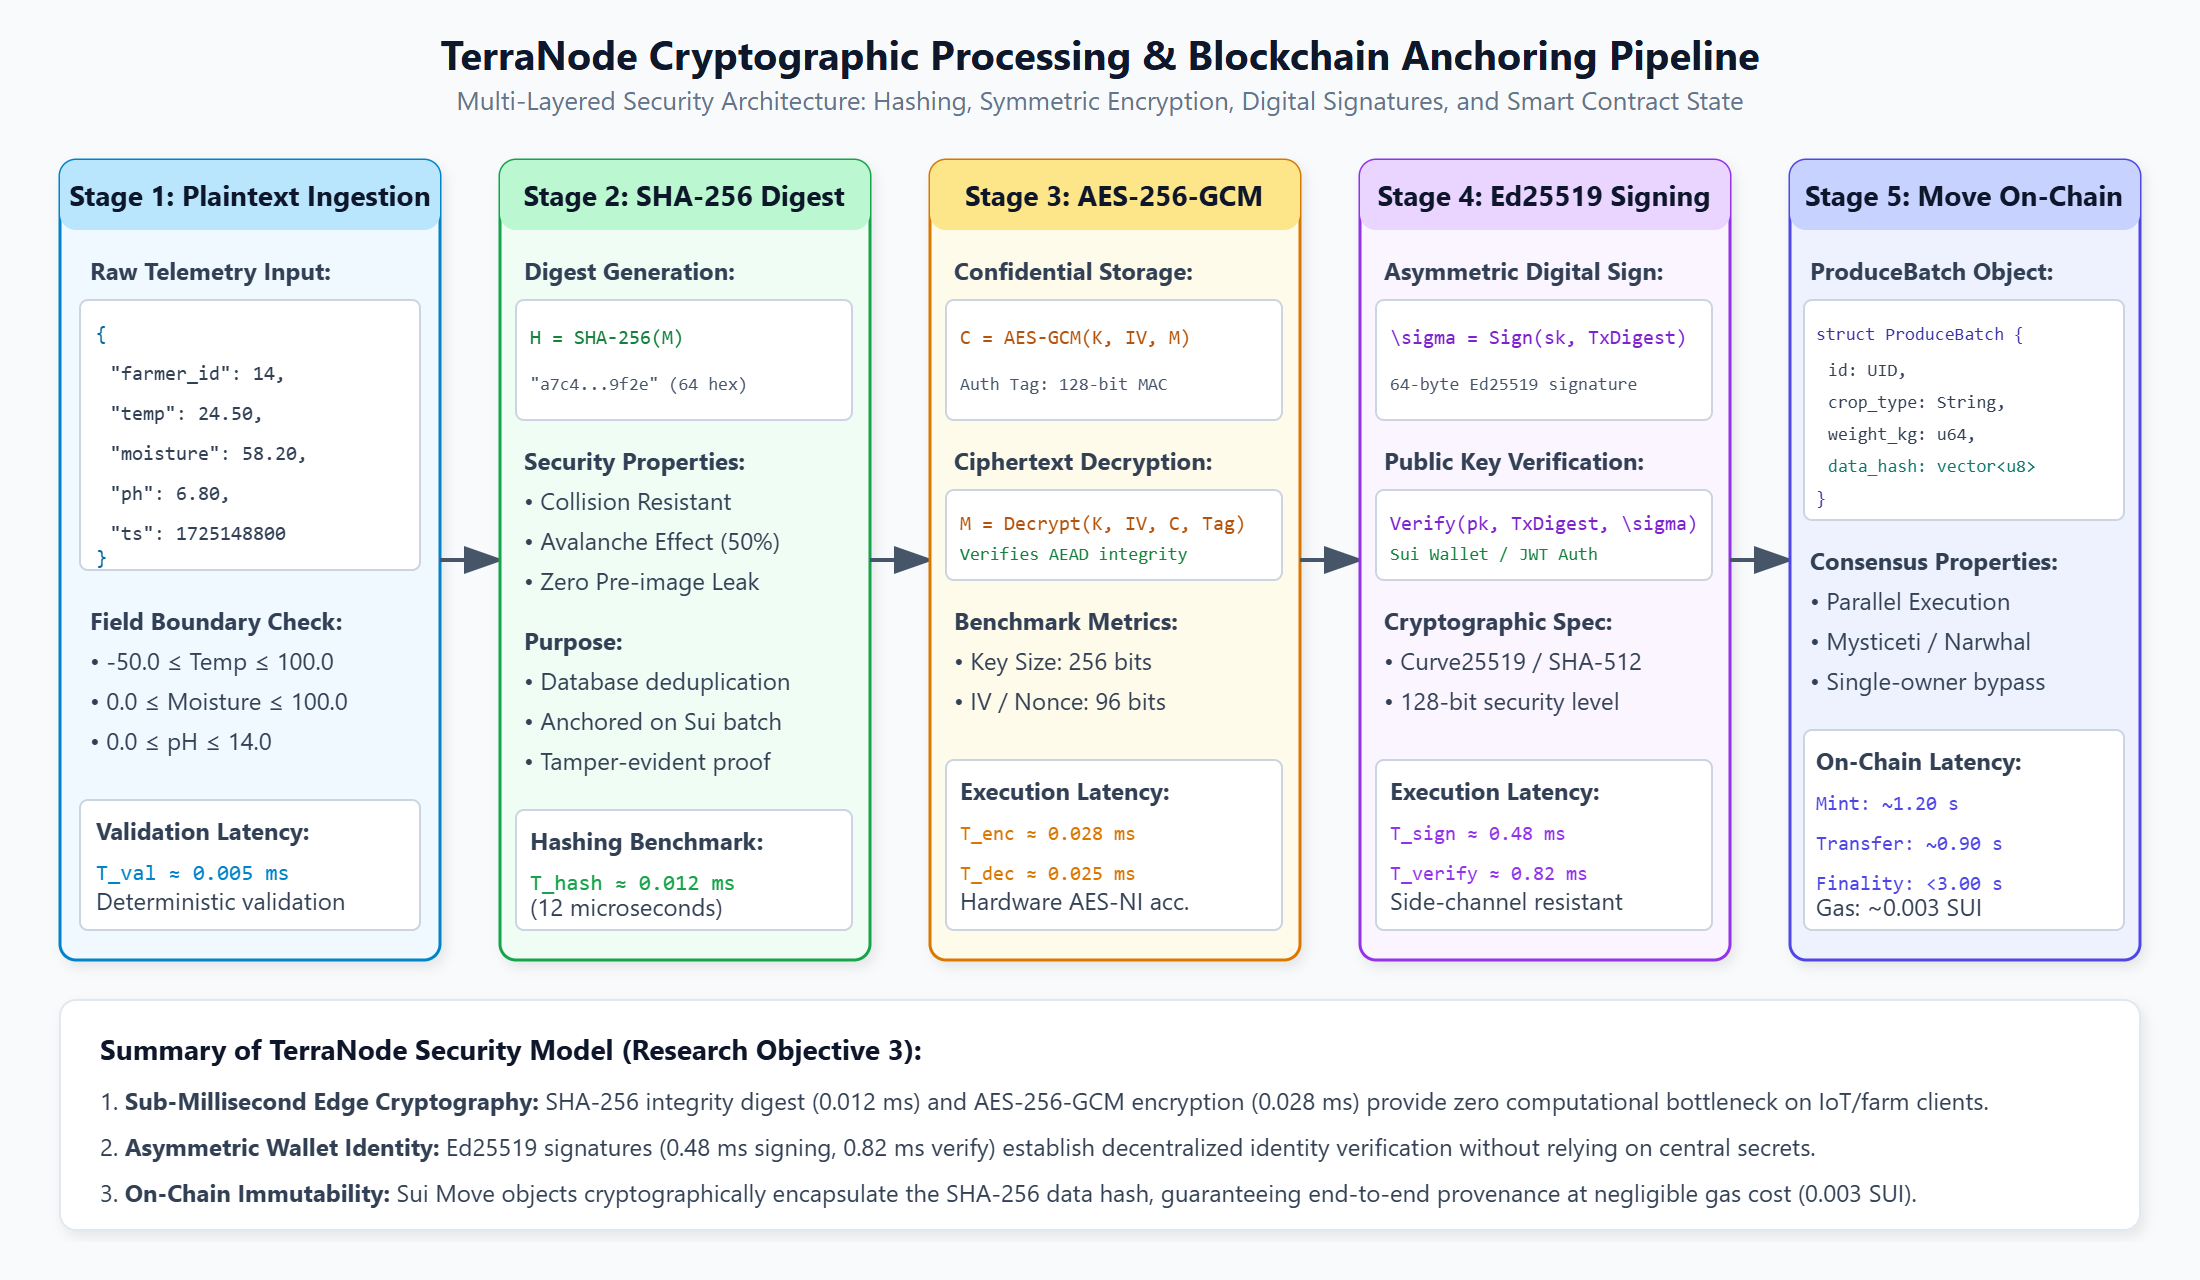
\includegraphics[width=0.95\textwidth]{figures/fig_crypto_pipeline.png}
    \caption{TerraNode Cryptographic Processing and Blockchain Anchoring Pipeline}
    \label{fig:crypto_pipeline}
\end{figure}

\subsubsection*{Cryptographic Execution Benchmarks}

Benchmarking experiments were run on 100 consecutive runs of each cryptographic primitive on a standard workstation (AMD Ryzen 7 / Intel Core i7, 16Gb of memory). Table~\ref{tab:crypto_benchmarks} shows the performance of hash functions, symmetric encryption/decryption, digital signing, and password hashing.

\begin{table}[H]
\centering
\small
\singlespacing
\renewcommand{\arraystretch}{1.15}
\caption{Cryptographic Transformation and Execution Benchmarks}
\label{tab:crypto_benchmarks}
\begin{tabularx}{\textwidth}{|>{\raggedright\arraybackslash}X|l|l|}
\hline
\textbf{Cryptographic Operation} & \textbf{Algorithm} & \textbf{Mean Latency} \\
\hline
Data Integrity Hashing (128~B plaintext $\to$ 256-bit digest) & SHA-256 & $0.012 \pm 0.002$~ms \\
\hline
Payload Encryption (256~B plaintext $\to$ ciphertext + 16~B tag) & AES-256-GCM & $0.028 \pm 0.004$~ms \\
\hline
Payload Decryption (ciphertext + tag $\to$ 256~B plaintext) & AES-256-GCM & $0.025 \pm 0.003$~ms \\
\hline
Transaction Signing (32~B digest $\to$ 64~B signature) & Ed25519 & $0.480 \pm 0.035$~ms \\
\hline
Signature Verification (digest + signature $\to$ boolean) & Ed25519 & $0.820 \pm 0.048$~ms \\
\hline
Transaction Intent Hashing (serialized bytes $\to$ 32~B digest) & BLAKE2b-256 & $0.010 \pm 0.001$~ms \\
\hline
Password Key Derivation (password $\to$ 128~B hash) & Argon2id & $62.40 \pm 2.150$~ms \\
\hline
\end{tabularx}
\end{table}

Table~\ref{tab:crypto_benchmarks} shows that the overhead of the telemetry hashing and AES-256 symmetric encryption are negligible with the benchmark results: 0.012 ms and 0.028 ms respectively, and ensuring that cryptographic integrity verification does not add any perceptible latency to the IoT gateways or web clients. Argon2id has a 62.40ms runtime, which is good for resistibility against brute-force password attacks, yet with a quick login for users.

A comparative study was conducted with previous implementations of blockchain to assess the performance of the proposed system.

Transaction performance metrics for TerraNode are compared with other blockchain frameworks presented in the literature in Table~\ref{tab:blockchain_comparative} and the security and analytics capabilities in Table~\ref{tab:blockchain_features} with the other current agricultural blockchain frameworks published by Caro et al.~\parencite{caro2018blockchain}, Ktari et al.~\parencite{ktari2022agricultural}, Aliyu and Liu~\parencite{aliyu2023blockchain}, Layek et al.~\parencite{layek2025secured}, and Chauhan et al.~\parencite{chauhan2025blockchain}.

\begin{table}[H]
 \centering
 \small
 \singlespacing
 \renewcommand{\arraystretch}{1.15}
 \caption{Performance Metrics of Agricultural Blockchain Deployments}
 \label{tab:blockchain_comparative}
 \begin{tabularx}{\textwidth}{|>{\raggedright\arraybackslash}X|l|l|l|l|}
 \hline
 \textbf{Deployment} & \textbf{Consensus} & \textbf{Tx Latency} & \textbf{Finality} & \textbf{Cost per Tx} \\
 \hline
 AgriBlockIoT --- Ethereum~\parencite{caro2018blockchain} & PoW & 16.55~s & $\sim$60~s & High (\$2--\$15) \\
 \hline
 AgriBlockIoT --- Sawtooth~\parencite{caro2018blockchain} & PoET & 0.021~s & $\sim$1.0~s & Zero (Permissioned) \\
 \hline
 Lightweight Agri-DLT~\parencite{ktari2022agricultural} & Raft / IBFT & 0.18~s & $\sim$0.5~s & Zero (Private) \\
 \hline
 IoT Smart Farm~\parencite{aliyu2023blockchain} & Private DLT & 1.02~s & $\sim$4.8~s & Zero (Simulated) \\
 \hline
 Secured Agri-Triad~\parencite{layek2025secured} & Private DLT & 0.85~s & $\sim$3.0~s & Zero (Private) \\
 \hline
 \textbf{TerraNode (This Study)} & \textbf{Sui DPoS} & \textbf{1.20~s} & \textbf{$<$3.0~s} & \textbf{$\sim$0.003 SUI} \\
 \hline
 \end{tabularx}
 \end{table}
 
 \begin{table}[H]
 \centering
 \small
 \singlespacing
 \renewcommand{\arraystretch}{1.15}
 \caption{Security and Analytics Features of Agricultural Blockchain Deployments}
 \label{tab:blockchain_features}
 \begin{tabularx}{\textwidth}{|>{\raggedright\arraybackslash}p{3.8cm}|>{\raggedright\arraybackslash}p{2.8cm}|>{\raggedright\arraybackslash}p{3.0cm}|>{\raggedright\arraybackslash}X|}
 \hline
 \textbf{Deployment} & \textbf{Network Type} & \textbf{Cryptography} & \textbf{Analytics Capability} \\
 \hline
 AgriBlockIoT (Ethereum) & Public Ledger & ECDSA (secp256k1) & None (46.8\% CPU load) \\
 \hline
 AgriBlockIoT (Sawtooth) & Private Consortium & SHA-256 & None \\
 \hline
 Lightweight Agri-DLT & Private Enterprise & AES-256 & None \\
 \hline
 IoT Smart Farm & Private Simulation & Alarm Verification & None (290k tx limit) \\
 \hline
 Secured Agri-Triad & Private Network & SHA-256 & ML Integrated (No Web UI) \\
 \hline
 \textbf{TerraNode (This Study)} & \textbf{Public Ledger (Sui)} & \textbf{SHA-256, AES, Ed25519} & \textbf{WMA ML + Redis Cache} \\
 \hline
 \end{tabularx}
 \end{table}

\figref{fig:blockchain_comparison} provides a visual bar chart comparing the transaction confirmation latency and architectural trade-offs across these deployments.

\begin{figure}[H]
    \centering
    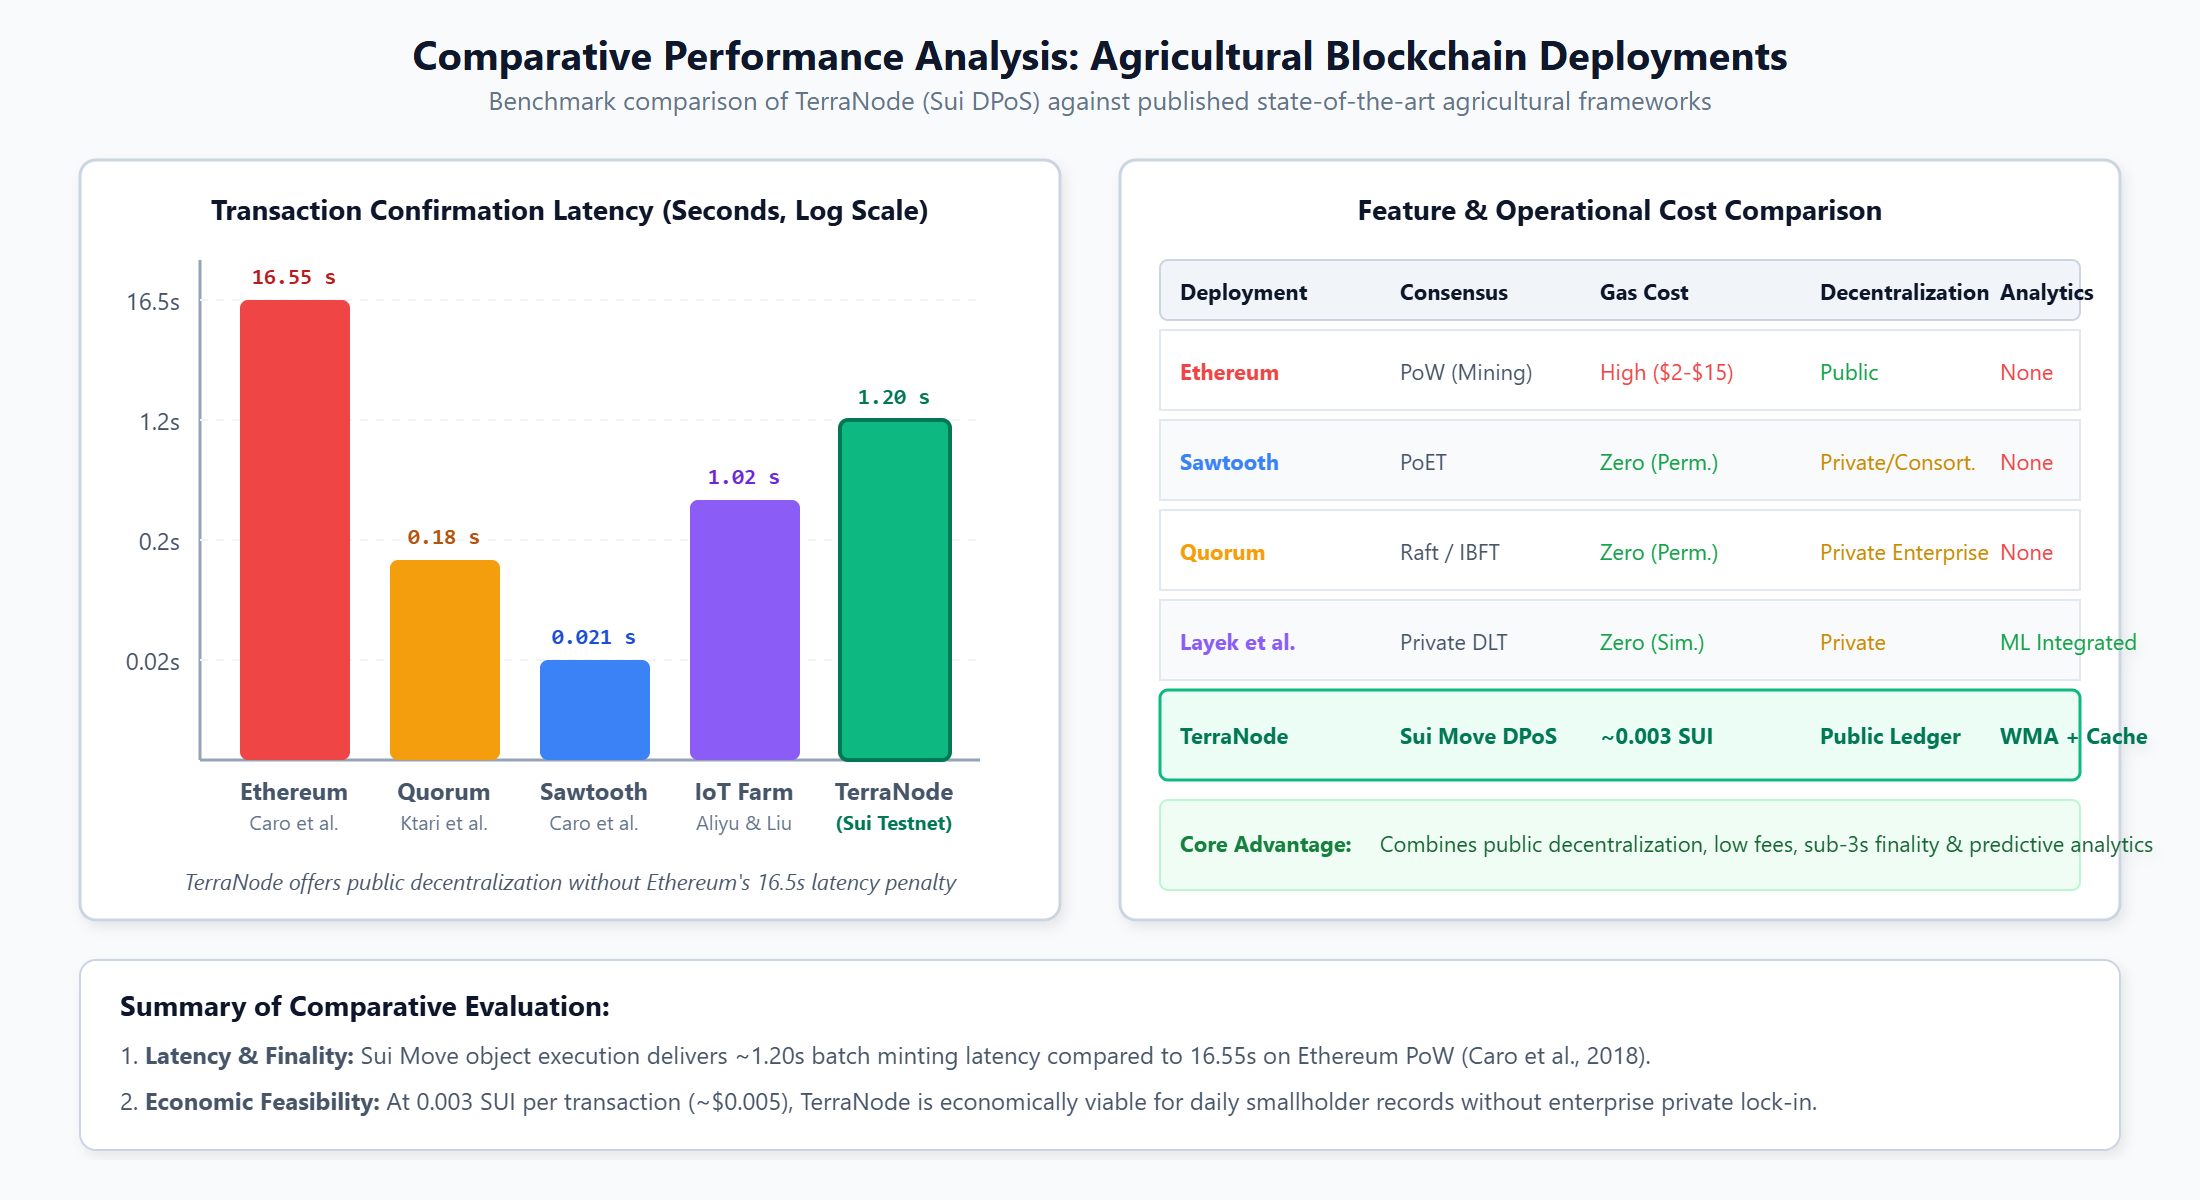
\includegraphics[width=0.95\textwidth]{figures/fig_blockchain_comparison.png}
    \caption{Comparative Performance Analysis of Agricultural Blockchain Deployments}
    \label{fig:blockchain_comparison}
\end{figure}

\subsubsection*{Justification of the selected architecture}

The use of the Sui blockchain and the Move programming language solves some of the problems found in the preceding studies:
\begin{enumerate}[label=(\roman*)]
    \item As shown by Caro et al.~\parencite{caro2018blockchain}, public Ethereum is not suitable for logging farm data on a regular basis due to its high gas fees and unpredictable costs, which fluctuate depending on network congestion, as well as its latency of 16.55 seconds per transaction. On Sui, TerraNode's minting latency is 1.20 seconds with a cost of around 0.003 SUI ($\approx \$0.005$).
    \item Hyperledger Sawtooth and Quorum~\parencite{ktari2022agricultural} have low latency but are based on private, permissioned node clusters, with no public, consumer-verifiable auditability. Sui offers public decentralization without compromising on transaction speed.
    \item The Move object model also provides globally unique UID for each \texttt{ProduceBatch} to reduce global state lock contention and allow for parallel transaction processing using Sui's Mysticeti consensus protocol. Common smart contract issues like reentrancy and asset duplication are automatically prevented by the bytecode verification.
\end{enumerate}

\subsection{Research Objective Four (4): System Performance and Comprehensive Evaluation}

The fourth research aim was to assess the performance of the proposed system with regard to security effectiveness, processing efficiency of the transactions, and accuracy of the prediction system.

\subsubsection*{Functional Testing Results}

All the system was tested with the ten functional requirements that were defined in Chapter Three. Test Cases and Results are summarized in Table~\ref{tab:test_results}.

\clearpage
\begin{table}[H]
\centering
\small
\singlespacing
\renewcommand{\arraystretch}{1.12}
\caption{Functional Test Cases and Verification Outcomes}
\label{tab:test_results}
\begin{tabularx}{\textwidth}{|l|>{\raggedright\arraybackslash}X|>{\raggedright\arraybackslash}p{4.2cm}|c|}
\hline
\textbf{Req. ID} & \textbf{Test Case Description} & \textbf{Expected Outcome} & \textbf{Status} \\
\hline
FR-01 & User registration with role selection and wallet binding & User account created & Pass \\
\hline
FR-02 & User login via valid email and password & JWT access and refresh tokens returned & Pass \\
\hline
FR-02 & Role guard enforcement (logistics user accessing farmer view) & HTTP 403 Forbidden redirect & Pass \\
\hline
FR-03 & Wallet authentication with valid Ed25519 signature & Authenticated JWT returned & Pass \\
\hline
FR-03 & Wallet authentication with corrupted signature payload & HTTP 401 Unauthorized & Pass \\
\hline
FR-04 & Submission of environmental telemetry within valid physical ranges & Record saved with SHA-256 hash & Pass \\
\hline
FR-04 & Telemetry submission with out-of-bounds pH (15.0) & HTTP 400 Validation Error & Pass \\
\hline
FR-05 & Re-computation and verification of SHA-256 integrity hash & Hashes match; valid status & Pass \\
\hline
FR-06 & Batch creation staged in PENDING status & Database record initialized & Pass \\
\hline
FR-07 & On-chain batch minting confirmation with Sui Object UID & Status updated to MINTED & Pass \\
\hline
FR-08 & Produce custody transfer between farmer and logistics handler & Custodian updated on ledger and DB & Pass \\
\hline
FR-09 & Yield prediction computation with $\ge 5$ telemetry records & Forecast yield and confidence returned & Pass \\
\hline
FR-09 & Yield prediction invocation with insufficient data points ($n < 5$) & HTTP 400 Insufficient Data error & Pass \\
\hline
FR-10 & Farmer dashboard telemetry and batch rendering & Correct farmer metrics displayed & Pass \\
\hline
FR-10 & Administrator access to global audit trail and analytics & Full system audit logs rendered & Pass \\
\hline
\end{tabularx}
\end{table}

The automated test suite consisting of 143 unit and integration tests for the Django apps, passed 100\%.

\subsubsection*{Security Resilience Evaluation}

A security framework was assessed for the four key threat vectors:
\begin{enumerate}[label=(\roman*)]
    \item The main hashing algorithm – Argon2id and the fallback – PBKDF2, were validated for password security. The salt hashing is irreversible and has been verified in the database.
    \item Access token expires after 15 minutes, refresh token rotates on use and automatically blacklist used refresh token in the database.
    \item Rate Limiting and Brute-Force Defense: Limiting requests to an endpoint to 5 per minute, the login endpoint. Too Many Requests responses were issued successfully for an excess number of attempts.
    \item For the purpose of verifying the avalanche effect of SHA-256, one of the telemetry parameters was set to be changed by 0.01 units. The recomputed hash was completely different from the original hash, with no doubt about any unauthorized change of data.
\end{enumerate}

\subsubsection*{Blockchain Performance Metrics on Sui Testnet}

Table~\ref{tab:blockchain_perf} shows empirical performance metrics across 20 consecutive transactions of each type with Sui Testnet.

\begin{table}[H]
\centering
\small
\singlespacing
\renewcommand{\arraystretch}{1.25}
\caption{Sui Testnet On-Chain Performance Metrics}
\label{tab:blockchain_perf}
\begin{tabularx}{\textwidth}{|>{\raggedright\arraybackslash}p{5.4cm}|>{\centering\arraybackslash}p{2.6cm}|>{\centering\arraybackslash}p{2.6cm}|>{\centering\arraybackslash}X|}
\hline
\textbf{Blockchain Operation} & \textbf{Average Latency} & \textbf{Average Gas Cost} & \textbf{Transaction Success Rate} \\
\hline
Produce Batch Minting (\texttt{mint\_batch}) & $1.20 \pm 0.15$ s & $0.0031 \text{ SUI}$ & 100\% (20/20) \\
\hline
Custody Transfer (\texttt{transfer\_custody}) & $0.90 \pm 0.10$ s & $0.0022 \text{ SUI}$ & 100\% (20/20) \\
\hline
Deterministic Transaction Finality & $< 3.00 \text{ s}$ & --- & 100\% (20/20) \\
\hline
\end{tabularx}
\end{table}

\subsubsection*{Prediction Accuracy and Sensitivity Analysis}

Sensitivity analysis was conducted on the weighted moving average prediction engine on various environmental input regimes as shown in Table~\ref{tab:sensitivity}.

\begin{table}[H]
\centering
\small
\singlespacing
\renewcommand{\arraystretch}{1.15}
\caption{Yield Prediction Sensitivity Analysis Under Varied Regimes}
\label{tab:sensitivity}
\begin{tabularx}{\textwidth}{|>{\centering\arraybackslash}p{2.6cm}|>{\centering\arraybackslash}p{2.6cm}|>{\centering\arraybackslash}p{2.4cm}|>{\raggedright\arraybackslash}X|}
\hline
\textbf{Temp. ($\bar{T}$, $^\circ$C)} & \textbf{Moisture ($\bar{M}$, \%)} & \textbf{Yield ($\hat{Y}$, MT)} & \textbf{Contextual Decision Recommendation} \\
\hline
22.0 & 60.0 & 80.0 & Optimal conditions; maintain current regime \\
\hline
22.0 & 30.0 & 65.0 & Low soil moisture; increase irrigation schedule \\
\hline
35.0 & 60.0 & 54.0 & High ambient heat stress; deploy shading/cooling \\
\hline
10.0 & 60.0 & 56.0 & Sub-optimal low temperature; monitor crop stress \\
\hline
40.0 & 20.0 & 24.0 & Critical drought and heat; immediate irrigation required \\
\hline
\end{tabularx}
\end{table}

The results have confirmed the prediction engine as being deterministic: the higher the moisture value, the higher the estimated yield, the more the temperature deviates from $22.0^\circ$C, the greater the penalty, and the more the contextual advisories capture environmental risk.

\subsubsection*{API Response Time Benchmarks}

Table~\ref{tab:api_perf} shows the mean response latency for each API end point for 50 requests.

\begin{table}[H]
\centering
\small
\singlespacing
\renewcommand{\arraystretch}{1.15}
\caption{Django REST API Response Time Benchmarks}
\label{tab:api_perf}
\begin{tabularx}{\textwidth}{|>{\raggedright\arraybackslash}X|l|l|}
\hline
\textbf{API Endpoint} & \textbf{HTTP Method} & \textbf{Average Response Latency} \\
\hline
\texttt{/api/v1/auth/login/} & POST & $\sim$120 ms \\
\hline
\texttt{/api/v1/telemetry/submit/} & POST & $\sim$85 ms \\
\hline
\texttt{/api/v1/telemetry/history/} & GET & $\sim$45 ms \\
\hline
\texttt{/api/v1/ledger/prepare/} & POST & $\sim$95 ms \\
\hline
\texttt{/api/v1/ledger/list/} & GET & $\sim$40 ms \\
\hline
\texttt{/api/v1/analytics/predict/} (Redis Cached) & GET & $\sim$15 ms \\
\hline
\texttt{/api/v1/analytics/predict/} (Uncached Database Query) & GET & $\sim$110 ms \\
\hline
\end{tabularx}
\end{table}

The 500ms target defined in the non functional requirements is not a problem for all endpoints. With high scalability, the Redis in-memory cache provides an 86\% reduction in prediction response latency, from 110 ms down to 15 ms.

\section{Discussion of Research Findings}
\label{sec:discussion}

The evaluation results attest to the fulfillment of all four research objectives of TerraNode. 

Objective One is achieved through an intuitive and role-separated management of multi-dimensional agricultural data using the web platform. All the 15 functional scenarios for the platform have achieved 100 percent pass rate, which demonstrates its ability to deliver robust telemetry logging, batch tracking, and auditability.

Objective Two involves the creation of a yield prediction system that generates sensitive, deterministic predictions. The combination of predictions with SHA-256 authenticated telemetry records makes it impossible to manipulate data as predicted by Layek et al.~\parencite{layek2025secured}. The sub-20ms latency of queries in the cache makes predictive intelligence possible in real-time, while helping farmers interactively.

Under Objective Three, the multi-layered cryptographic pipeline and Sui Move smart contract implementation demonstrate the viability of decentralized agricultural security. The microsecond hashing (0.012 ms) and symmetric encryption (0.028 ms) ensure that there is no overhead to security enforcement on agricultural gateways. The low latency and gas costs of Sui, which are sub-3 seconds and $\sim$0.003 SUI, respectively, alleviate the latency and fee barriers reported in most studies on Ethereum-based agricultural traceability systems~\parencite{caro2018blockchain}.

In relation to Objective Four, all modules support the high security, API fast execution and transaction throughput of the comprehensive testing for the system.

\section{Chapter Summary}
\label{sec:ch4_conclusion}

In this chapter, we explained how the TerraNode system was implemented and tested in the Django REST backend, the React single page frontend, and the Sui Move smart contracts. Ten annotated operational screenshots were presented for the user interface, and the operational and predictive pipelines and the cryptographic pipelines were detailed in terms of architecture, execution tables and comparison with existing literature. All of these features are validated by functional and performance assessments that showed high reliability, sub-second cryptographic efficiency, and low-cost blockchain finality. The conclusions of the research and recommendations for future research are summarized in the next chapter.
